\documentclass{beamer}
\usepackage{times, amsthm, amsmath, amssymb, cancel, changepage, graphicx, lipsum, fancyhdr, mathabx,caption, subcaption}
\usetheme{CambridgeUS}
\usecolortheme{seagull}
\usefonttheme{serif}
\definecolor{navy}{RGB}{0, 0, 128} 
\setbeamercolor{frametitle}{fg=navy}
\setbeamercolor{title}{fg=navy}
\setbeamerfont{frametitle}{series=\bfseries}
\setbeamerfont{title}{series=\bfseries}

\title{\textbf{Lecture 12: Change of Variables I}}
\date{October 3, 2019}

\begin{document}
	
\frame{\titlepage}


\begin{frame}
\frametitle{Review of Single Variable Case}
In the univariate case we have:
$$\int_a^b f(g(x))g'(x)dx = \int_{g(a)}^{g(b)} f(u) du$$
Where
\begin{itemize}
	\item[(i)] $g'(x)$ is continuous on $[a,b]$.
	\item[(ii)] $f(x)$ is continuous on a range of $g$.
	\item[(iii)] $u=g(x)$ is the transformation
\end{itemize}
This process is also called u-substitution.\\
\vspace{12pt}
\textbf{Example:}
\begin{itemize}
	\item[(a)] $\int_0^4 \sqrt{3x+4} \, dx$
\end{itemize}
\end{frame}

\begin{frame}
\frametitle{Transformations in Two Variables}
\begin{figure}
	
	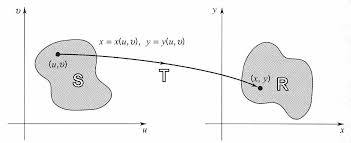
\includegraphics[width=.9\textheight]{vmap.jpg}\\
	\hspace*{10pt}\hbox{\thinspace{\tiny\itshape ksuweb.kenneshaw.edu}}
\end{figure}
We consider a change of variables given by the transformation $T$ from the $(u,v)$ plane to the $(x,y)$ plane.
$$\iint\limits_R f(x,y) dx\,dy = \iint\limits_S g(u,v)dv\,du$$
\end{frame}


\begin{frame}
\frametitle{Transformations}
\setbeamertemplate{itemize items}[ball]
\begin{itemize}
	\item A function $F$ that maps $\mathit{R}^2 \rightarrow \mathit{R}^2$ is called "one-to-one" if $\forall (u,v)$ in the domain of $F$ on the $(u,v)$ plane, $\exists$ only one $(x,y)$ in the $(x,y)$ plane.
	\item The transformation $T$ is given by $$T(u,v) = (x,y) \mbox{ or } x=g(u,v), y=h(u,v)$$
	\item If $T(u,v) = (x,y)$, then $(x_1,y_1)$ is the image of $(u_1,v_1)$ under the transformation $T$. If no two points have the same image, $T$ is one-to-one.
	\item $T$ is a $C^1$ transformation which means that $g$ and $h$ have continuous 1st order partials.
\end{itemize}
\end{frame}


\begin{frame}
\frametitle{Transformations}
\begin{figure}
	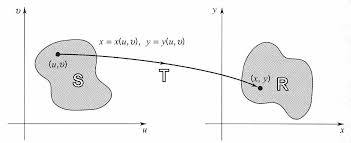
\includegraphics[width=.8\textheight]{vmap.jpg}\\
	\hspace*{10pt}\hbox{\thinspace{\tiny\itshape ksuweb.kenneshaw.edu}}
\end{figure}

\begin{itemize}
	\item $T$ transforms $S$ into a region $R$ in the $(x,y)$ plane called the image of $S$.
	\item $T$ is said to be "onto" $R$ if each point in $R$ is the image of some point in $S$.
	\item A transformation $T$ that is one-to-one and onto is invertable, denoted by $T^{-1}$.
	$$T^{-1}(x,y) = (u,v) \mbox { or } u = G(x,y), v=H(x,y)$$
\end{itemize}
\end{frame}

\begin{frame}
\frametitle{Is $T$ Invertible?}
How do you tell if $T$ is invertible 
\begin{itemize}
	\item[(1)] Given that $x = g(u,v)$ and $y=h(u,v)$, take all the partial derivatives of $x$ and $y$ with respect to $u$ and $v$.
	\item[(2)] Form the Jacobian, $J = |M|$, of the transformation which is the determinate of the matrix
	$$M = \begin{bmatrix}
		\frac{\partial x}{\partial u} & 	\frac{\partial x}{\partial v}\\
			\frac{\partial y}{\partial u} & 	\frac{\partial y}{\partial v}
	\end{bmatrix} \mbox{ giving } J=|M| = \frac{\partial x}{\partial u} \frac{\partial y}{\partial v}-	\frac{\partial x}{\partial v}\frac{\partial y}{\partial u} $$
	\item[(3)] If $J \neq 0$ then $T^{-1}$ exists.
\end{itemize}
\textbf{Example:}
\begin{itemize}
	\item[(a)] $T$ is given by $x=u^2-v^2$ and $y=2uv$. If $S = \{ (u,v)| 0\leq u \leq 1, 0\leq v\leq1\}$. Is $T$ invertible?
\end{itemize}
\end{frame}


\begin{frame}
\frametitle{Finding the Image of $S$ Under $T$}
How do we find $R$?
\begin{itemize}
	\item Need to find new limits of integration
	\item Process is to work along the boundaries of $S$ and determine what happens on the $(x,y)$ plane.
\end{itemize}
\textbf{Example:}
\begin{itemize}
	\item[(a)] $T$ is given by $x=u^2-v^2$ and $y=2uv$. If $S = \{ (u,v)| 0\leq u \leq 1, 0\leq v\leq1\}$. Find region $R$.
	\item[(b)] $T$ is given by $u=x+y$ and $v=x-y$. If $R = \{ (x,y)| 0\leq x \leq 1, 0\leq y\leq1\}$. Find region $S$.
\end{itemize}
\end{frame}

\begin{frame}
\frametitle{Change of Variables Formula}
If the following applies:
\begin{itemize}
	\item[(i)] $T$ is invertible. (Namely $J \neq 0$.)
	\item [(ii)] $T$ is $C^1$.
	\item[(iii)] $T$ maps region $S$ in $(u,v)$ plane onto region $R$ in $(x,y)$ plane.
	\item[(iv)] $f$ is continuous in $R$.
	\item[(v)] $R$ and $S$ are Type I or Type II regions
\end{itemize}
\vspace{12pt}
Then we can apply the change of variables formula:
$$\iint\limits_{R} f(x,y)dy\,dx = \iint\limits_{S} f[g(u,v),h(u,v)] |J| dv\,du$$

\textbf{Example:}
\begin{itemize}
	\item[(a)] $T$ is given by $x=u^2-v^2$ and $y=2uv$. If $S = \{ (u,v)| 0\leq u \leq 1, 0\leq v\leq1\}$. Express and evaluate the integral $\iint\limits_{R} y dy\,dx$ in terms of $(u,v)$.
\end{itemize}
\end{frame}
\end{document}
